\section{Wireframes}
Let's now look at how our solution will look to the user.
\todo[inline]{add figure numbers}
Figure x contains a mockup of the guest profile editor application.
The user selects what allergens they want to avoid in their food.
Then they can choose from some of the most popular diets which they follow.
After that they can specify what food ingredients they like and dislike by writing their name to the corresponding input field and clicking the "Add" button.
When the user is finished with creating their profile, they click the "Save" button at the bottom of the screen to save their profile.

\begin{figure}[h]
  \centering
  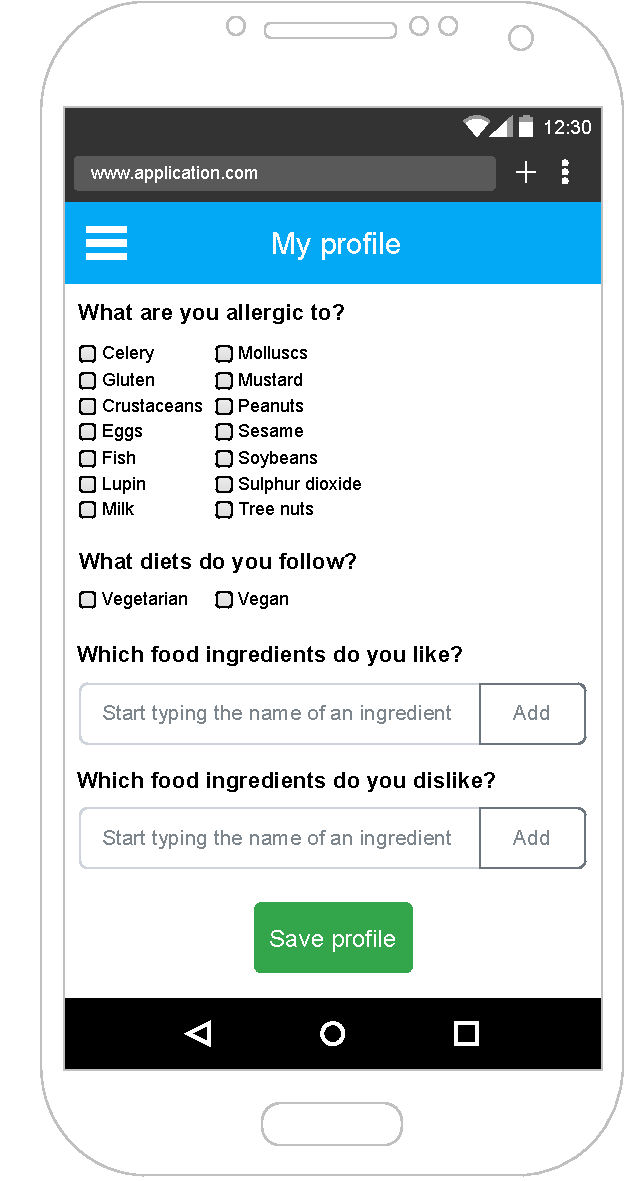
\includegraphics[width=0.62\linewidth]{master-thesis/img/wireframes/dietary_profile_editor.pdf}
  \caption{The guest profile editor application}
\end{figure}

Figure x shows what will the restaurant employee see when they log in to the restaurant menu maker application.
The screen contains a list of previously created menus by the restaurant employee.
Each menu can be viewed, edited or deleted by pressing the corresponding buttons.
The restaurant employee can create a new menu by pressing the "Create a new menu" button.

\begin{figure}[h]
  \centering
  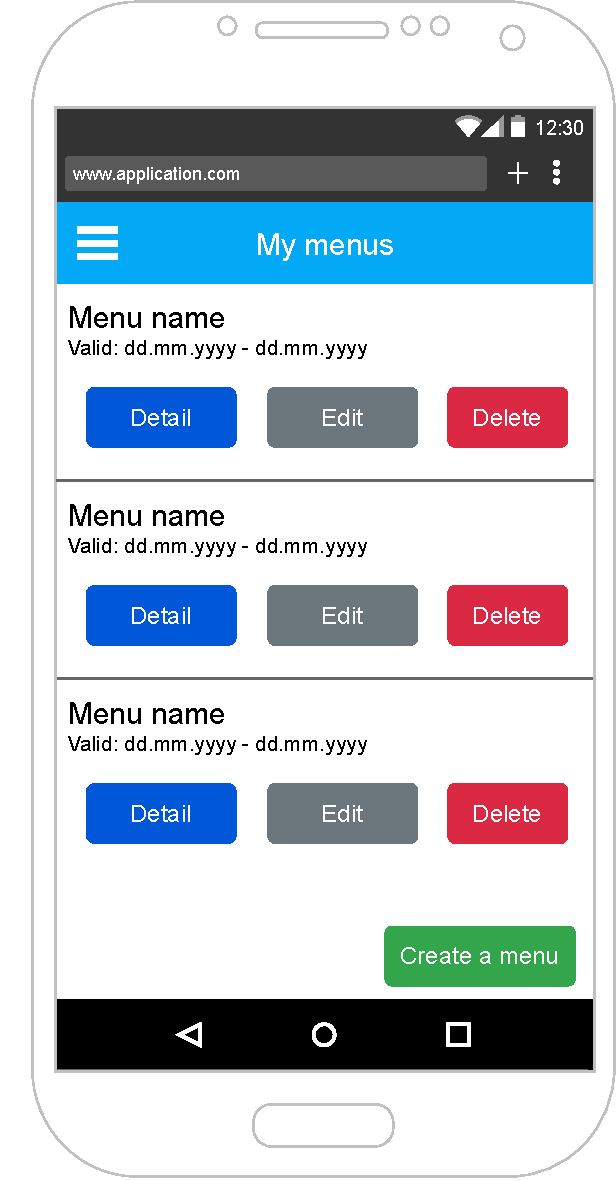
\includegraphics[width=0.62\linewidth]{master-thesis/img/wireframes/menu_creator_menus_overview.pdf}
  \caption{The menus overview screen of the restaurant menu maker application}
\end{figure}

Figure x contains a mockup of the screen which is displayed when a restaurant employee is creating a new menu.
They can specify the menu's name and date when it will be valid.
The restaurant employee can populate the menu by either creating a new item or reusing a previously created item.

\begin{figure}[h]
  \centering
  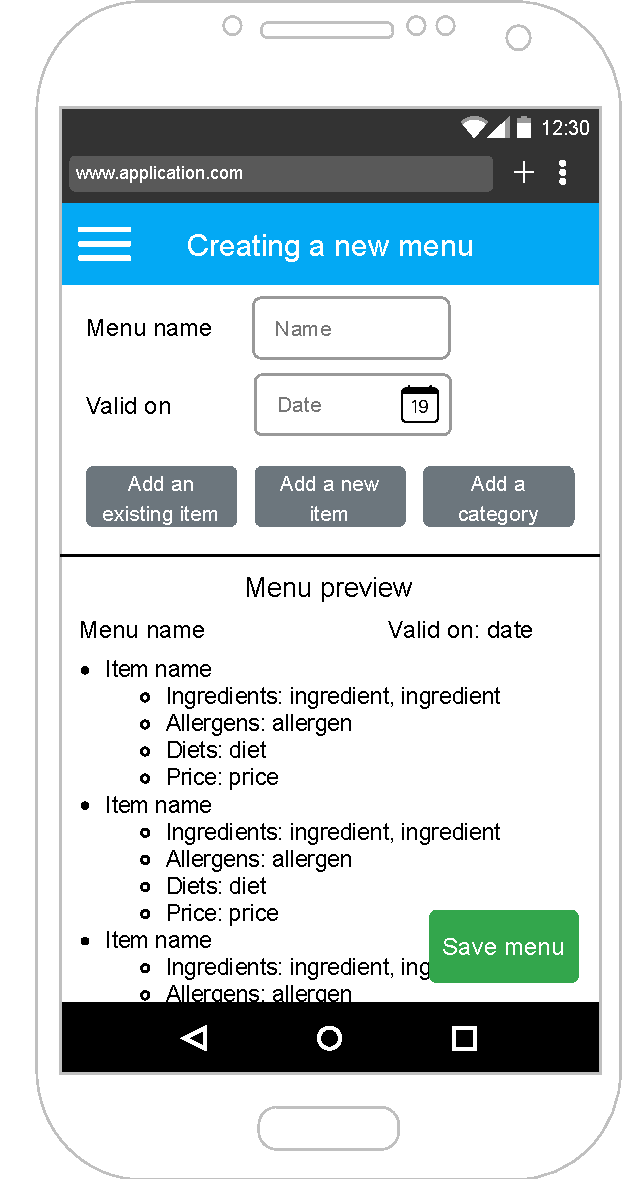
\includegraphics[width=0.62\linewidth]{master-thesis/img/wireframes/menu_creator_new_menu.pdf}
  \caption{The new menu screen of the restaurant menu maker application}
\end{figure}

Figure x shows a screen which is displayed when a restaurant guest logs in to the personalized menu viewer application.
It contains an overview of currently served foods by the guest's favorite restaurants.
A detail of a menu can be displayed upon clicking an "Open menu" button.

\begin{figure}[h]
  \centering
  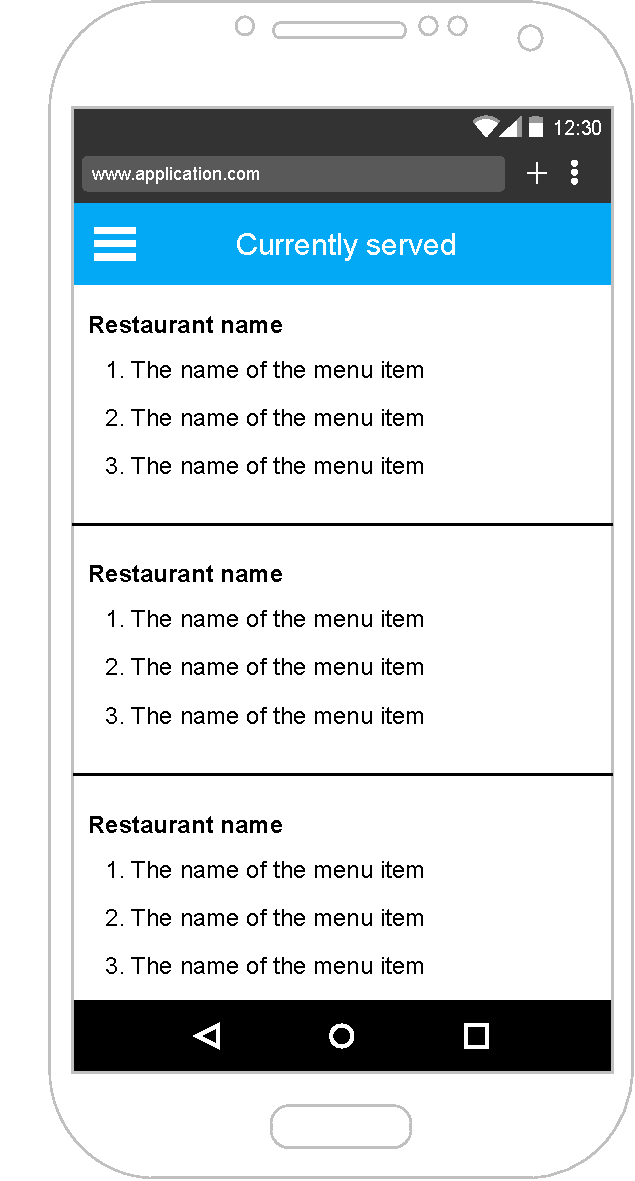
\includegraphics[width=0.62\linewidth]{master-thesis/img/wireframes/menu-viewer-currently-served.pdf}
  \caption{The personalized menu viewer application's home page}
\end{figure}

A detail of a menu can be seen in figure x.
The menu is divided into two sections.
The first section contains the items which the guest can eat.
The second section contains the items which the guest cannot eat and within each item, the reason why the guest should avoid the food is highlighted, e.g. that it contains a certain allergen which the guest is allergic to.

\begin{figure}[h]
  \centering
  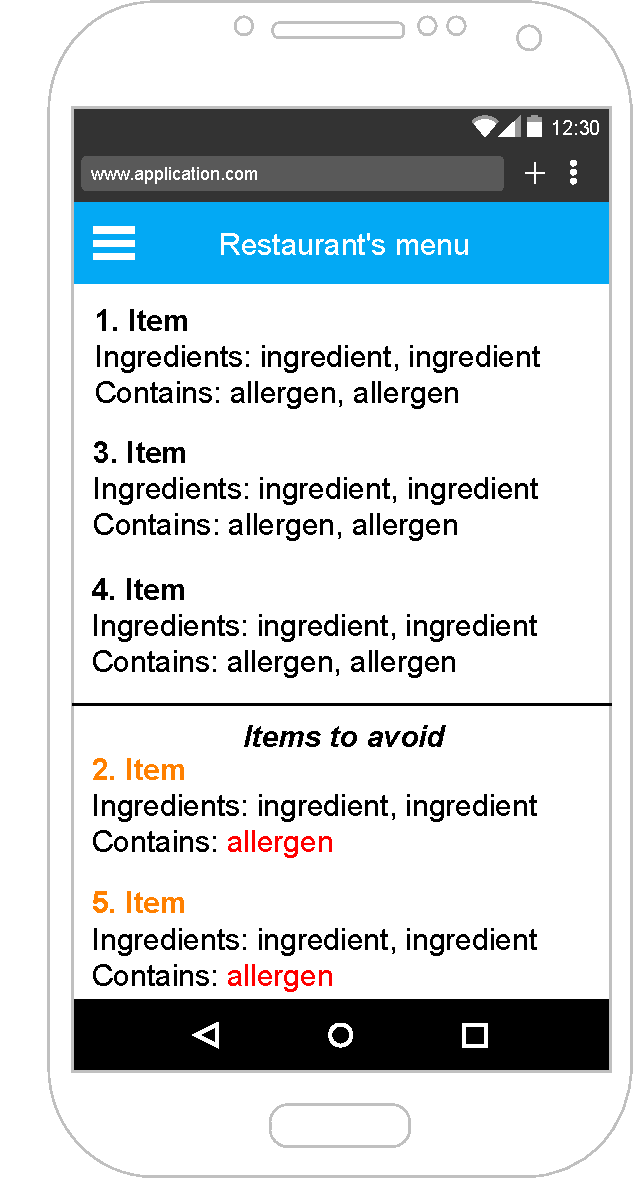
\includegraphics[width=0.62\linewidth]{master-thesis/img/wireframes/menu_viewer_menu_detail.pdf}
  \caption{The personalized menu viewer application's menu detail}
\end{figure}
